 \let\negmedspace\undefined
\let\negthickspace\undefined
\documentclass[journal]{IEEEtran}
\usepackage[a5paper, margin=10mm, onecolumn]{geometry}
%\usepackage{lmodern} % Ensure lmodern is loaded for pdflatex
\usepackage{tfrupee} % Include tfrupee package

\setlength{\headheight}{1cm} % Set the height of the header box
\setlength{\headsep}{0mm}     % Set the distance between the header box and the top of the text

\usepackage{gvv-book}
\usepackage{gvv}
\usepackage{cite}
\usepackage{amsmath,amssymb,amsfonts,amsthm}
\usepackage{algorithmic}
\usepackage{graphicx}
\allowdisplaybreaks
\usepackage{textcomp}
\usepackage{xcolor}
\usepackage{txfonts}
\usepackage{listings}
\usepackage{enumitem}
\usepackage{mathtools}
\usepackage{gensymb}
\usepackage{comment}
\usepackage[breaklinks=true]{hyperref}
\usepackage{tkz-euclide} 
\usepackage{listings}
% \usepackage{gvv}                                        
\def\inputGnumericTable{}                                 
\usepackage[latin1]{inputenc}                                
\usepackage{color}                                            
\usepackage{array}                                            
\usepackage{longtable}                                       
\usepackage{calc}                                             
\usepackage{multirow}                                         
\usepackage{hhline}                                           
\usepackage{ifthen}                                           
\usepackage{lscape}
\begin{document}

\bibliographystyle{IEEEtran}
\vspace{3cm}

\title{1-1.5-27}
\author{AI24BTECH11002 - K.AKSHAY TEJA}
% \maketitle
% \newpage
% \bigskip
{\let\newpage\relax\maketitle}

\renewcommand{\thefigure}{\theenumi}
\renewcommand{\thetable}{\theenumi}
\setlength{\intextsep}{10pt} % Space between text and floats


\numberwithin{equation}{enumi}
\numberwithin{figure}{enumi}
\renewcommand{\thetable}{\theenumi}

\textbf{Question:}\\
 If the coordinates of points $\vec{A}$ and $\vec{B}$ are \brak{-2,-2} and \brak{2,-4} respectively, find the coordinates of $\vec{P}$ such that $AP = \frac{3}{7} AB$, and $\vec{P}$ lies on the line segment $AB$. 
 
    \hfill {(10, 2015)}

 \solution
 \begin{table}[h!]
	 \centering
	 \input{Tables/Table.tex} 
	\caption{Coordinates of points $A$ and $B$}
	 \label{tab:Coordinates}
\end{table}

Given, $AP = \frac{3}{7} AB$.That means $P$ divides $AB$ in ratio 3:4\\

Using section formula, 
\begin{align}
	\vec{P}&=\frac{1}{1 + k}\myvec{\vec{A} & \vec{B}}\myvec{1 \\ k}\\[5pt]
	\vec{P}&=\frac{1}{1+\frac{3}{4}}\myvec{-2 & 2\\-2 & -4}\myvec{1 \\ \frac{3}{4}}\\[5pt]
	\vec{P}&=\frac{4}{7}\myvec{\frac{-1}{2} \\[2 pt] -5}\\[5pt]
	&=\myvec{\frac{-2}{7} \\[2pt] \frac{-20}{7}}
\end{align}
	\newpage
	\begin{figure}[h!]    
	  \begin{center}
		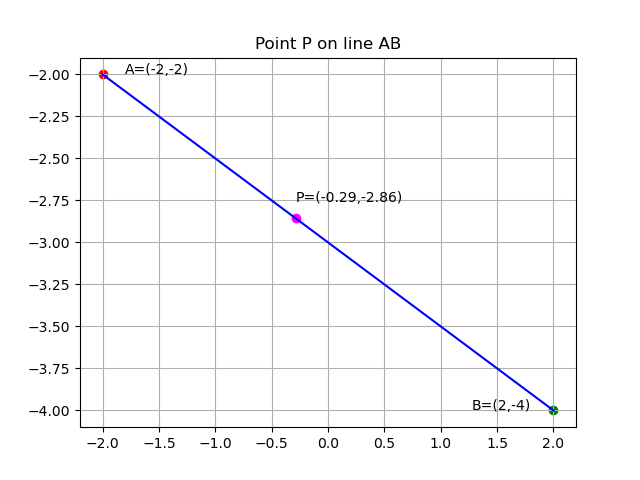
\includegraphics[width=0.7\textwidth]{Figs/Fig.png}
		\label{Graph}
		  \caption{Plot of points A,B and P}  
	 \end{center}	  
	\end{figure}

\end{document}

